%% ----------------------------------------------------------------
%% 3_Chapter3.tex
%% ----------------------------------------------------------------
\chapter{Requirements and Analysis} \label{Chapter:three}

This chapter will analyse the requirements of the proposed application and inform the design decisions that have been made.

\section{Use cases}
Explanation

    \begin{figure}
        \center
        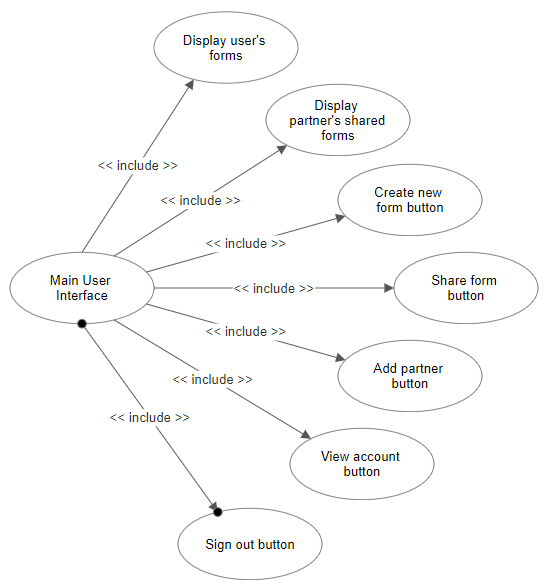
\includegraphics{../figures/UseCaseInterface}
        \caption{Use Case Diagram 1}
    \end{figure}

    \begin{figure}
        \center
        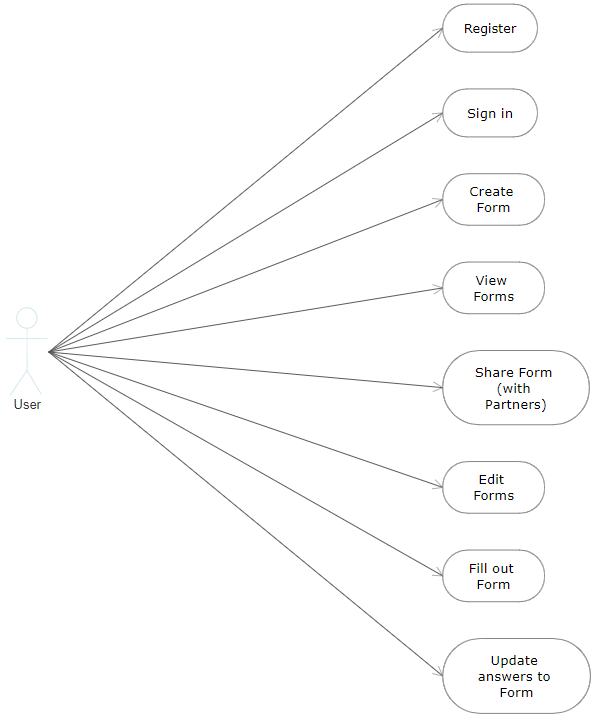
\includegraphics[scale=0.70]{../figures/UseCaseUser}
        \caption{Use Case Diagram 2}
    \end{figure}

    \subsection{Use case description}

        The following table explains the major use cases for the application.

        \begin{table}[b]
            \centering
            \begin{tabular}{|c|c|}
                \hline
                Use Case & Description\\
                \hline
                \hline
                Display user's forms & \makecell{A list of forms created by the user will be displayed, with\\the form's name, owner and date of last modification.}\\
                \hline
                \makecell{Display partner's\\shared form} & \makecell{A list of forms shared with the user by a partner will be\\displayed, with the form's name, owner and date of\\last modification.}\\
                \hline
                \makecell{Create new\\form button} & Takes the user to a page where they can design a new form.\\
                \hline
                Share form button & \makecell{Allows the user to share forms they have created with\\partners.}\\
                \hline
                Add partner button & \makecell{Allows the user to search for other people's accounts on\\the application, and add them as partners. This should\\be done with other users that one would wish to share\\ forms with and/or receive forms from.}\\
                \hline
                View account button & \makecell{Allows the user to view their account information and edit\\it if necessary. Details such as name, email, company\\and the abilityto change the account's password.}\\
                \hline
                Sign out button & Allows the user to sign out from the application.\\
                \hline
            \end{tabular}
            \caption{Use case descriptions}
        \end{table}

\section{Functional requirements}
Explanation

\begin{table}[h]
    \centering
    \begin{tabular}{|c|c|}
        \hline
        Requirement & Description\\
        \hline
        \hline
        Register & \makecell{New users will create an account before being allowed to use\\the application.}\\
        \hline
        Log in & \makecell{Users will need to log in before they are able to\\access their account, create, share and complete forms.}\\
        \hline
        Create a form & \makecell{Users will be able to create a new form, which will be saved to\\their account.}\\
        \hline
        Share a form & \makecell{Users will be able to share a form that they have created with\\a partner.}\\
        \hline
        Add a partner & \makecell{Users will be able to view and edit their account information,\\including; name, email, company and password (not viewable).}\\
        \hline
        Sign out & Users will be able to sign out of the application.\\
        \hline
        Notifications & \makecell{Users will be notified of various changes, including their partners'\\answers to forms.}\\
        \hline
    \end{tabular}
    \caption{Functional requirements}
\end{table}

\begin{table}[h]
    \centering
    \begin{tabular}{|c||c|c|c|c|c|}
        \hline
        Complexity/Time & Low & Medium & High\\
        \hline
        \hline
        Short & 0.0625 & 0.125 & 0.25\\
        \hline
        Medium & 0.125 & 0.25 & 0.5\\
        \hline
        Long & 0.25 & 0.5 & 0.75\\
        \hline
    \end{tabular}
    \caption{Importance Levels}
\end{table}

\begin{table}[h]
    \centering
    \begin{tabular}{|c|c|c|c|}
        \hline
        Requirement & Complexity & Time & Importance Level\\
        \hline
        \hline
        Register & Medium & Short & 0.125\\
        \hline
        Log in & Low & Short & 0.0625\\
        \hline
        Create a form & Medium & Medium & 0.25\\
        \hline
        Share a form & High & Medium & 0.5\\
        \hline
        Add a partner & Medium & Medium & 0.25\\
        \hline
        Sign out & Low & Low & 0.0625\\
        \hline
        Notifications & Medium & Short & 0.125\\
        \hline
    \end{tabular}
    \caption{Requirements analysis}
\end{table}

\section{Non-functional requirements}
Explanation\\table

\begin{table}
    \centering
    \begin{tabular}{|c|c|}
        \hline
        Requirement & Description\\
        \hline
        \hline
        Internet connection & \makecell{The application will be hosted online, therefore users will require\\a connection to the internet in order to access the application.}\\
        \hline
    \end{tabular}
    \caption{Non-functional requirements}
\end{table}

\section{Risk analysis}
Explanation\\tables

\begin{table}
    \centering
    \begin{tabular}{|c||c|c|c|c|c|}
        \hline
        Consequence/Likelihood & Negligible & Minor & Moderate & Major & Catastrophic\\
        \hline
        \hline
        Impossible & 0 & 0 & 0 & 0 & 0\\
        \hline
        Low & 0 & 0.0625 & 0.125 & 0.1875 & 0.25\\
        \hline
        Medium & 0 & 0.125 & 0.25 & 0.375 & 0.5\\
        \hline
        High & 0 & 0.1875 & 0.375 & 0.5625 & 0.75\\
        \hline
        Certain & 0 & 0.25 & 0.5 & 0.75 & 1\\
        \hline
    \end{tabular}
    \caption{Risk Levels}
\end{table}

\begin{table}
    \centering
    \begin{tabular}{|c|c|c|c|c|c|}
        \hline
        Risk & Likelihood & Consequence & Risk Rating & Mitigation\\
        \hline
        \hline
        Network loss & High & Minor & 0.1875 & Frequent update of database.\\
        \hline
        Data loss & Low & Catastrophic & 0.25 & Redundant database.\\
        \hline
        Security breach & Low & Catastrophic & 0.25 & \makecell{Follow good practice for secure\\deveopment of cloud applications.}\\
        \hline
        Function error & Medium & Major & 0.375 & \makecell{Implementation of test\\framework to ensure application\\is fully functional.}\\
        \hline
        Interface error & Medium & Major & 0.375 & \makecell{Implementation of test\\framework to ensure application\\is fully functional.}\\
        \hline
    \end{tabular}
    \caption{Risk Analysis}
\end{table}

\section{Functionality}

\begin{figure}[]
\center
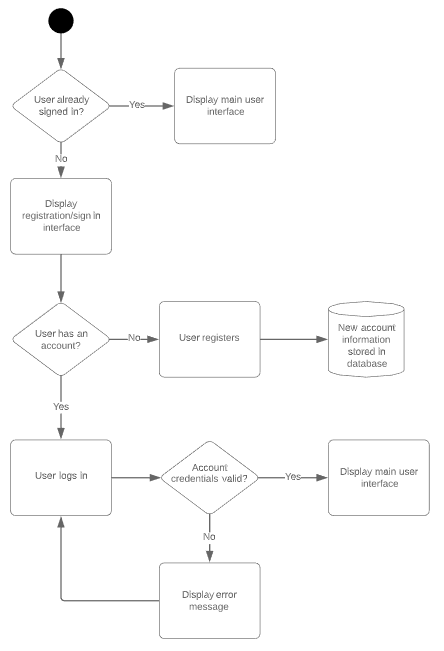
\includegraphics{../figures/ActivityDiagramAuthentication}
\caption{Activity Diagram: Authentication}
\end{figure}

\begin{figure}[]
\center
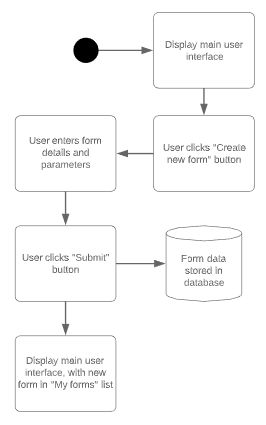
\includegraphics{../figures/ActivityDiagramFormCreation}
\caption{Activity Diagram: Form Creation}
\end{figure}

\begin{figure}[]
\center
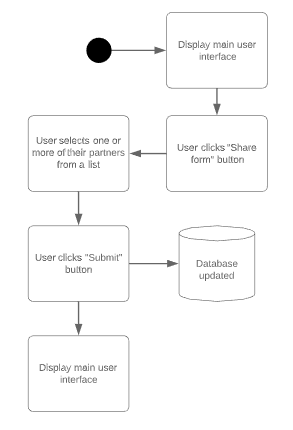
\includegraphics{../figures/ActivityDiagramFormSharing}
\caption{Activity Diagram: Form Sharing}
\end{figure}

\begin{figure}[]
\center
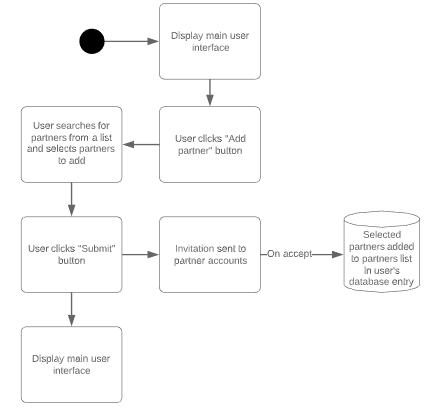
\includegraphics{../figures/ActivityDiagramPartnerInvitation}
\caption{Activity Diagram: Partner Invitation}
\end{figure}

\section{Justification of the Approach (?)}